\newpage
\section{Revisão Teórica}
\subsection{Modulação BFSK}
A modulação FSK ("\emph{Frequency Shift Keying}") é uma técnica de modulação que consiste em variar a frequência da portadora em função do sinal modulante, no caso o sinal digital a ser transmitido.
Pode-se considerar que este tipo de modulação é equivalente a modulação FM analógica \cite{couch}.

A amplitude da onda portadora modulada é mantida constante durante todo o processo de modulação, quando o sinal digital apresenta nível lógico "1" a frequência da portadora é alterada para posteriormente ser detectada no processo de demodulação.
A frequência resultante transmitida será a frequência da onda portadora $f_c$ diminuida de uma frequência de desvio $f_d$ \cite{taufik1}.
Ou seja
\begin{equation}
    f_r = f_c - f_d
\end{equation}

Para a ocorrência de um nível lógico "0", a frequência resultante será a frequência da portadora mais a frequência de desvio.
\begin{equation}
    f_r = f_c + f_d
\end{equation}

\begin{figure}[H]
    \centering
    \caption{Modulação FSK}
    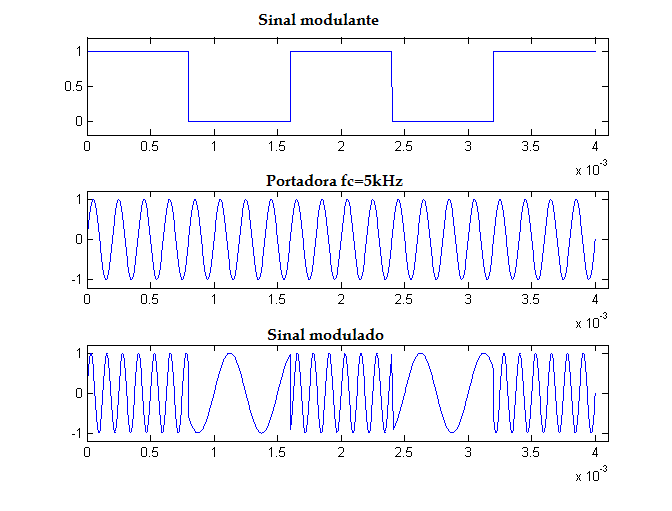
\includegraphics[scale=0.9]{fsk.png}
    \label{fig:mdfsk}
    
    \small Fonte: Abrão, T. (2016).
\end{figure}

A Figura \ref{fig:mdfsk} mostra um sinal modulante, uma portadora $f_c=5kHz$ com $f_d = 3kHz$.
É possível observar um sinal em $8kHz$ quando o sinal modulante é "1" e em $2kHz$ quando o sinal modulante é "0", ou seja, o esquema FSK se utiliza da frequência como um meio de transportar a informação, sendo que, para cada frequência $f_i$, é mapeado um simbolo $s_i$.

A largura de banda utilizada na transmissão de sinais modulados em FSK é \cite{abrao}:
\[
BW = 2\cdot \Delta f +2B.
\]

Onde $BW$ é a largura de banda ocupada, $\Delta f$ é a variação de frequência para representar os bits e $B$ é a banda ocupada desde  $f_c + \Delta f$ até o primeiro nódulo da onda \textit{sinc}, a qual representa o espectro de um nível do sinal. 
Esse fato fica evidente ao analisarmos a Figura \ref{fig:bw}, a qual mostra o espectro de um sinal FSK.

\begin{figure}[H]
    \centering
    \caption{Espectro de uma sinal modulado com FSK.}
    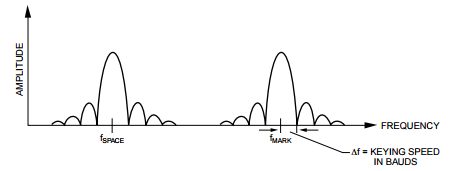
\includegraphics[scale=0.9]{bw}
    \label{fig:bw}
    
    \small Fonte: Wikipedia, 2016.
\end{figure}

\subsection{Circuito modulador FSK}

A Figura \ref{fig:modulador} representa o diagrama de blocos de um modulador FSK, onde um sinal de mensagem entra em \textit{Digital Signal} e, através do VCO (\textit{Voltage Controled Oscillator}), modifica a frequência da onda de saída. A frequência da portadora, $f_c$, é dada por um circuito que pode ser feito com um resistor e um capacitor, os quais determinam o período de oscilação da frequência central.

\begin{figure}[H]
    \centering
    \caption{Modulador FSK com VCO.}
    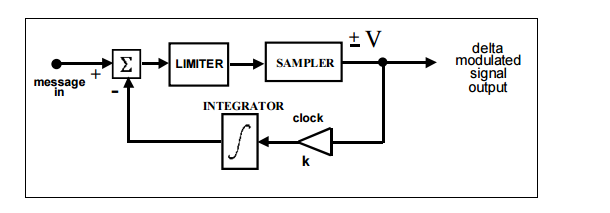
\includegraphics[scale=0.5]{modulador}
    \label{fig:modulador}
    
    \small Fonte: Wikipedia, 2016.
\end{figure}

\subsection{Circuito demodulador}

O detector utilizado é um detector não-coerente, ou seja, que não possui as informações de fase e frequência da portadora. O método escolhido para a demodulação é através de um PLL, o qual rastreia a frequência do sinal recebido de forma a ser aplicada no detector.



\begin{figure}[H]
    \centering
    \caption{Detector coerente com PLL.}
    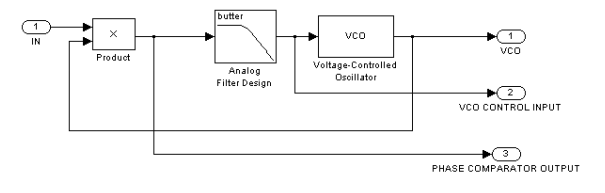
\includegraphics[scale=0.5]{coerente}
    \label{fig:detector}
    
    \small Fonte: Wikipedia, 2016.
\end{figure}

O funcionamento do circuito da Figura \ref{fig:565} é melhor entendido se analisarmos o diagrama de blocos da Figura \ref{fig:detector}. Nesta imagem é possível ver que o trabalho do CI 565 consiste em extrair as informações de fase e frequência do sinal transmito, de modo a produzir, com um VCO, um sinal semelhante, o qual é utilizado como referência para aplicação no detector coerente.

Desta forma é possível obter na saída a representação binaria do dado transmitido.

\newpage